\section{基于分隔集的分块}
\label{sec:graph-separator-blocks}

大图上的计算常常希望“分而治之”：把图拆成几块分别处理，再在块与块的连接处汇总。第~\ref{sec:graph-connectivity-separation}节定义了分隔集：删除一个顶点集$S$后，若某些顶点之间不再有路径，$S$就把它们分隔开。本节接受一个给定的候选集$S$，用连通分量计算检验它是否真的把图拆成了几侧，再把$S$加回各侧，得到共享接口的局部块。本节只负责结构上的分块：怎样找到好的分隔集不在这里讨论，块上的数值怎样沿接口组合则放在第~\ref{chap:graph-dynamic-programming}章。

\subsection{删除集合后的分量}
\label{sec:graph-trav-delete-separator}

\paragraph{输入、输出与三种结果}
输入是无向图$\mathcal G=(V,E)$和一个候选集合$S\subseteq V$。删除$S$中的顶点及与它们关联的边，得到$\mathcal G-S$，即$V\setminus S$上的诱导子图；对它计算连通分量$C_1,\ldots,C_r$。不同的$C_j$之间在$\mathcal G-S$中没有边，所以原图中从$C_j$到$C_k$（$j\neq k$）的任何路径都必须经过$S$。按$r$的取值有三种结果：$r\geq2$时，$S$把图拆成了$r$侧，任取两个不同分量中的顶点，$S$都把它们分隔开；$r=1$时，删除$S$后其余顶点仍然连通，$S$没有形成多侧拆分；$r=0$时$S=V$，余图为空，也谈不上拆分。是否拆分成功只能由计算结果判断，不能因为输入被称作“分隔集”就默认成立。

\begin{algorithm}[删除候选集后的分量]
\label{alg:graph-trav-separator-components}
输入：无向图的邻接表，候选集合$S\subseteq V$。输出：$\mathcal G-S$的连通分量$C_1,\ldots,C_r$，以及拆分是否成功（$r\geq2$）。
\begin{enumerate}
  \item 用一个布尔数组标记$S$中的顶点为“屏蔽”，不修改原邻接表。
  \item 对未屏蔽的顶点执行算法~\ref{alg:graph-trav-components}：外层扫描跳过屏蔽顶点，遍历时读到屏蔽的邻居一律跳过。
  \item 输出各分量；若$r\geq2$报告拆分成功，$r=1$报告未拆分，$r=0$报告余图为空。
\end{enumerate}
\end{algorithm}

\paragraph{贯穿图上的检验}
在贯穿四点图上取$S=\{2,3\}$。删除$2,3$后，与它们关联的边$\{1,2\}$、$\{1,3\}$、$\{2,3\}$、$\{2,4\}$、$\{3,4\}$全部消失，只剩顶点$1$和$4$，而$\{1,4\}$不是原图的边，所以余图有两个分量$\{1\}$与$\{4\}$，见图~\ref{fig:graph-trav-separator-blocks}(a)。$S=\{2,3\}$成功地分隔了$1$和$4$。作为对照，取$S=\{1\}$，删除后剩下的$2,3,4$两两相邻，构成一个三角形，余图只有一个分量，见图~\ref{fig:graph-trav-separator-blocks}(c)，$\{1\}$不是有效的拆分。贯穿图中删去任何单个顶点都不会断开余图：删去$1$或$4$剩下三角形，删去$2$或$3$剩下一条路径，所以它没有割点，至少要删两个顶点才能拆开。

\paragraph{检验与优化是两个问题}
上面的计算回答的是“这个给定的$S$是否拆开了图”，用$O(n+m)$时间就能完成。它不回答“最小的拆分集合是什么”。若想通过检验来找最小的分隔集，就要逐个尝试候选集合：大小为$k$的候选集有$\binom{n}{k}$个，每个都要做一次连通分量计算，规模稍大就无法承受。寻找小的分隔集需要另外的方法，它们不是一次连通标记能自动给出的。

\subsection{局部块与公共接口}
\label{sec:graph-trav-blocks-interfaces}

\paragraph{把接口加回各侧}
删除$S$之后，各分量之间不再相连；但原图中分量内的顶点与$S$之间的边、$S$内部的边也随之丢失了。要把原图完整地分成几块，需要把$S$加回每一侧，得到\term{局部块}（local block）
\[
\mathcal B_j=\mathcal G[C_j\cup S],\qquad j=1,\ldots,r,
\]
其中$S$称为各块的公共接口。图~\ref{fig:graph-trav-separator-blocks}(b)中两个局部块是$\mathcal G[\{1,2,3\}]$与$\mathcal G[\{2,3,4\}]$，都是三角形，共享顶点$2,3$和边$\{2,3\}$。

\begin{figure}[!htb]
  \centering
  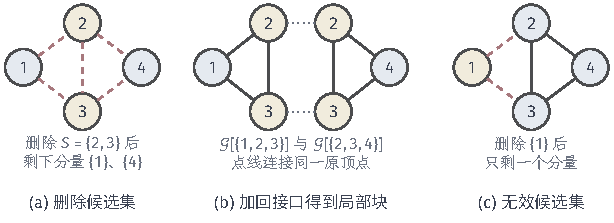
\includegraphics[width=103.9mm]{figures/01-basic-mathematics/04-graphs/tikz/c2-separator-blocks/figure.pdf}
  \caption{基于分隔集的分块。黄色顶点为候选删除集，红色虚线为随之删去的边。(a)贯穿四点图删除$S=\{2,3\}$后剩下两个分量$\{1\}$与$\{4\}$；(b)把$S$加回各侧得到两个局部块，两块中的$2,3$是同一批原顶点（点线相连），边$\{2,3\}$被两块共同引用；(c)删除$\{1\}$后余下三角形仍然连通，没有形成拆分。}
  \label{fig:graph-trav-separator-blocks}
\end{figure}

局部块覆盖了原图的每一条边。原图的一条边有三种可能：两端都在某个$C_j$中，或一端在$C_j$、一端在$S$中，这两种边都属于$\mathcal B_j$；两端都在$S$中，这样的边属于每一个块。由于不同分量之间没有边，不存在第四种情况。因此，原图的全部信息都保存在这些块中，块与块之间只通过$S$发生联系。

\paragraph{共享引用与复制}
不同局部块中的接口顶点是同一批原顶点，而不是可以各自独立变化的副本。若以后要给顶点赋值，同一个接口顶点在各块中必须取相同的值；若块中记录了边的数据，$S$内部的边被多个块同时看到，汇总时不能重复计数。因此表示局部块时，应保存接口顶点和接口边的唯一身份，各块只引用它们，而不是把原图的一部分真正复制几份后各自修改。

\paragraph{计算与存储开销}
屏蔽$S$并计算余图分量需要$O(n+m)$时间。输出局部块的存储另计：各块顶点数之和为$\sum_j(|C_j|+|S|)=(n-|S|)+r|S|$，接口顶点被重复列出$r$次；$S$内部的边也在每个块中出现一次。$r$和$|S|$都较小时，这部分额外存储可以忽略；接口很大或块很多时，就应采用共享引用。

\paragraph{小接口不保证块内简单}
接口小，只说明块与块之间的联系少，并不说明每个块内部简单。例如两个各有$100$个顶点的完全图只共用一个顶点，删除这个顶点就把图拆成两侧，接口大小为$1$，可每个局部块仍是一个$100$个顶点的完全图。分块的收益取决于后续计算在块内需要做什么。第~\ref{chap:graph-dynamic-programming}章会看到，当计算由许多只涉及少数顶点的局部项组成时，固定接口上的取值后各块可以分别处理，这时接口大小直接决定中间表的规模；那里还会把一次分块推广为多层的树分解。
